\documentclass{article}
\usepackage{tikz}
\usetikzlibrary{calc, patterns}
\usepackage{amsmath}

\begin{document}

\title{Double Pendulum Dynamics}
\author{}
\date{}
\maketitle

\section{Single Pendulum}
Our single pendulum model will consist of a point mass of mass $m$ connected to a pivot by a massless rod of length $l$. The angle of the rod with respect to the vertical is defined as $\theta$.
\begin{figure}[h]
    \centering
    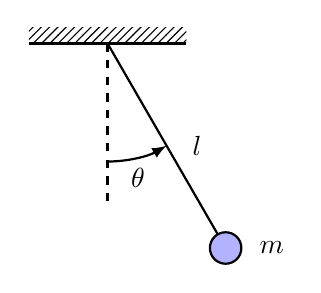
\begin{tikzpicture}[thick, >=latex]
        \def\Lone{3}
        \def\thetaone{30}
        \def\r{0.2}

        \coordinate (O) at (0,0);
        \coordinate (M) at ({\Lone * sin(\thetaone)}, {-\Lone * cos(\thetaone)});

        \fill [pattern = north east lines] (-1, 0) rectangle (1,0.2);
        \draw (-1, 0) -- (1, 0);

        \draw[dashed] (O) -- ++(0,-2);

        \draw (O) -- (M) node[midway, right= 0.2cm] {$l$};

        \filldraw[fill=blue!30] (M) circle (\r) node[right=0.3cm] {$m$};

        \draw[->] (0,-1.5) arc (-90:{-90+\thetaone}:1.5) node[midway, below] {$\theta$};
    \end{tikzpicture}
    \caption{Single Pendulum}
\end{figure}

\begin{figure}[h]
    \centering
    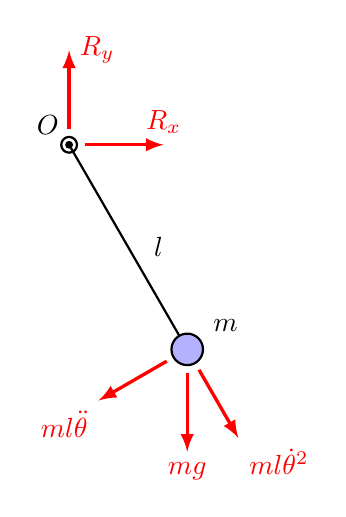
\begin{tikzpicture} [thick, >=latex]
        \def\Lone{3}
        \def\thetaone{30}
        \def\r{0.2}

        \coordinate (O) at (0,0);
        \coordinate (M) at ({\Lone * sin(\thetaone)}, {-\Lone * cos(\thetaone)});

        \draw (O) -- (M) node[midway, right= 0.2cm] {$l$};

        \fill (O) circle (0.05);
        \draw[thick] (O) circle (0.1) node[above left] {$O$};

        \filldraw[fill=blue!30] (M) circle (\r) node[above=0.3cm, right=0.2cm] {$m$};

        \draw[->, red, very thick] ($(O)+(0.2,0)$) -- ++(1,0) node[above] {$R_x$};
        \draw[->, red, very thick] ($(O)+(0,0.2)$) -- ++(0,1) node[above, right] {$R_y$};
        
        \draw[->, red, very thick] ($(M)+(0,-0.3)$) -- ++(0,-1) node[below] {$mg$};
        \draw[->, red, very thick] ($(M)+(\thetaone+180:0.3)$) -- ++(\thetaone+180:1) node[below left] {$ml\ddot{\theta}$};
        \draw[->, red, very thick] ($(M)+(\thetaone-90:0.3)$) -- ++(\thetaone-90:1) node[below right] {$ml\dot{\theta}^2$};
        
        
    \end{tikzpicture}
    \caption{Free Body Diagram of Single Pendulum}
\end{figure}



\section{System Description}
The double pendulum consists of two masses $m_1$ and $m_2$ attached by rigid massless rods of lengths $l_1$ and $l_2$.

\begin{figure}[h]
    \centering
    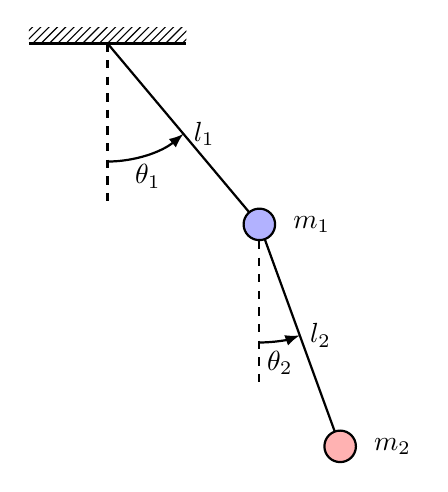
\begin{tikzpicture}[thick, >=latex]
        % Parameters
        \def\Lone{3}
        \def\Ltwo{3}
        \def\thetaone{40} % degrees
        \def\thetatwo{20} % degrees
        \def\r{0.2} % ball radius

        % Coordinates
        \coordinate (O) at (0,0);
        \coordinate (M1) at ({\Lone*sin(\thetaone)}, {-\Lone*cos(\thetaone)});
        \coordinate (M2) at ($(M1) + ({\Ltwo*sin(\thetatwo)}, {-\Ltwo*cos(\thetatwo)})$);

        % Ceiling
        \fill [pattern = north east lines] (-1,0) rectangle (1,0.2);
        \draw[thick] (-1,0) -- (1,0);

        % Vertical dashed lines for angles
        \draw[dashed] (O) -- ++(0,-2);
        \draw[dashed] (M1) -- ++(0,-2);

        % Rods
        \draw[thick] (O) -- (M1) node[midway, right] {$l_1$};
        \draw[thick] (M1) -- (M2) node[midway, right] {$l_2$};

        % Masses
        \filldraw[fill=blue!30] (M1) circle (\r) node[right=0.3cm] {$m_1$};
        \filldraw[fill=red!30] (M2) circle (\r) node[right=0.3cm] {$m_2$};

        % Angles
        % Angle 1
        \draw[->] (0,-1.5) arc (-90:{-90+\thetaone}:1.5) node[midway, below] {$\theta_1$};
        % Angle 2
        \draw[->] ($(M1) + (0,-1.5)$) arc (-90:{-90+\thetatwo}:1.5) node[midway, below] {$\theta_2$};

    \end{tikzpicture}
    \caption{Double Pendulum Diagram showing lengths $l_1, l_2$, masses $m_1, m_2$, and angles $\theta_1, \theta_2$.}
    \label{fig:double_pendulum}
\end{figure}

\end{document}
